\documentclass[11pt, a4paper]{article}
\usepackage[utf8]{inputenc}
\usepackage[english]{babel}
\usepackage{amsmath}
\usepackage{amsfonts}
\usepackage{amssymb}
\usepackage{graphicx}
\usepackage{tikz}
\usepackage{listings}
\usepackage[justification=centering]{caption}
\usetikzlibrary{arrows, automata, graphs, shapes, petri, decorations.pathmorphing}

\renewcommand{\labelenumi}{(\roman{enumi})}

\author{Niklas Rieken}
\title{Äquivalenzsatz von Kleene und Pumping-Argumente}


\begin{document}
\maketitle

In diesem Dokument geht es um die Äquivalenz von regulären Ausdrücken und endlichen Automaten. Stephen C. Kleene zeigte, dass es zu jedem regulären Ausdruck einen DFA(!) gibt und umgekehrt. Der Beweis damals war aufgrund des fehlenden Konzept des \textit{Nichtdeterminismus} ziemlich abgedreht (denkt mal drüber nach, wie man es anstellt aus einem Regexp sofort einen DFA zu bauen). Zum Schluss zeigen wir noch wie man beweisen kann, dass eine Sprache nicht regulär ist über ein sogenanntes Pumping-Argument. Es ist nicht genau das Pumping-Lemma, was in der Vorlesung meist recht ausführlich behandelt wird. Stattdessen beweisen wir etwas direkter, dass für eine nicht-reguläre Sprache kein endlicher Automat existieren kann. Das Dokument entstand aus einem Übungsblatt des Sommersemesters 2016.

\subsection*{Reguläre Ausdrücke}
Reguläre Ausdrücke sind induktiv aufgebaut und beschreiben immer eine reguläre Sprache, welche mit den FA-erkennbaren Sprachen zusammenfallen (Satz von Kleene).\par
Reguläre Ausdrücke sind wie folgt definiert:\\
Basisfälle: \( \emptyset, \varepsilon \) und \( a \) sind reguläre Ausdrücke für jedes \( a \in \Sigma \).\\
Rekursionsschritt: Sind \( r \) und \( e \) reguläre Ausdrücke, so sind auch \( (r \cdot e), (r + e) \) und \( r^\ast \) reguläre Ausdrücke.\\
Semantisch stehen die Ausdrücke \( \emptyset, \varepsilon, a \) für die Sprachen \( L(\emptyset) := \emptyset, L(\varepsilon) := \{ \varepsilon \}, L(a) := \{ a \} \) und im rekursiven Fall \( L(r \cdot e) := L(r) \cdot L(e), L(r + e) := L(r) \cup L(e), L(r^\ast) := L(r)^\ast \). Klammern und \( \cdot \) werden gerne auch weggelassen, wenn der Ausdruck auch so klar ist.\par
Gelegentlich kennen Studenten reguläre Ausdrücke bereits durch Programme wie \texttt{grep, sed, vim}, womit sich Textdateien u.a. durchsuchen lassen mithilfe von POSIX-Ausdrücken. Diese sind gleichmächtig mit denen aus der Vorlesung, sollten aber nicht verwendet werden. Man möchte die Anzahl der Rekursionen auf das Minimum reduzieren, da dadurch auch die Beweise über reguläre Ausdrücke kürzer werden. Auf POSIX-Shortcuts wie \( (r?) \) für \( (r + \varepsilon) \), Umbenennungen wie \( (r|e) \) für \( (r + e) \) oder Schreibweisen wie \( [a-c] \) für \( (a + b + c) \) solltet ihr also verzichten. Die einzige Ausnahme ist hier vielleicht \( r^+ \) für \( rr^\ast \).\par
Aus den Tutoraufgaben hier zwei Beispiele nun:
\begin{description}
	\item[a)] \( L_1 = \{ w \in \{ a, b, c \}^\ast \,\vert\, w \text{ hat gerade Länge } \} \).\\
		\( r_1 = ((a+b+c)(a+b+c))^\ast \). Das dieser Ausdruck die Sprache beschreibt lässt sich wie gewohnt über Induktion beweisen (zwei Richtungen für Gleichheit). Das ist aber hier nicht gefordert.
	\item[c)] \( L_3 = \{ w \in \{ a, b, c \}^\ast \,\vert\, \left| w \right| > 0 \text{ und } w \text{ beginnt und endet mit dem selben Symbol} \} \).\\
		\( r_3 = a(a+b+c)^\ast a + b(a+b+c)^\ast b + c(a+b+c)^\ast c + a + b + c \). Hier werden die Spezialfälle für \( \left| w \right| = 1 \) gerne übersehen.
\end{description}
Statt \( (a+b+c) \) schreibt man gerne auch einfach \( \Sigma \). Das ist aber eigentlich nicht ganz korrekt, da wir zwischen regulären Ausdrücken und den Sprachen die sie beschreiben unterscheiden. (\( r \) vs. \( L(r) \)). Streng genommen sind demnach auch die Zeichen \( \emptyset, \varepsilon, a \), wie oben in der Definition der regulären Ausdrücke, verschieden von den der Sprache \( \emptyset \), dem leeren Wort \( \varepsilon \) und dem Symbol \( a \in \Sigma \). Wenn man also wie in Aufgabe a) z.B. \( (\Sigma\Sigma)^\ast \) schreiben möchte, sollte man sich zumindest vorher \( \Sigma \) als regulären Ausdruck \( \Sigma := (a+b+c) \) definieren.


\subsection*{Von Automaten zu regulären Ausdrücken (Floyd-Warshall-Algorithmus)}
Das Verfahren was hier beschrieben wird ist leider ziemlich umständlich und technisch (im Vergleich zum Vorjahr), es ist aber das von Prof. Grohe präferierte Verfahren, deshalb müssen wir da jetzt durch. Die Idee ist eigentlich sogar recht einfach: Wir wollen vom Startzustand \( q_0 \) alle möglichen Pfade (d.h. über alle möglichen Zustände) zu akzeptierenden Zuständen finden (hier nur \( q_0 \)). Allgemein suchen wir den regulären Ausdruck
\[
	r = \sum_{q \in F} r_Q(q_0, q) = r_Q(q_0, p_1) + \ldots + r_Q(q_0, p_k),
\]
wobei \( p_1, \ldots, p_k \in F \). Die Notation funktioniert folgendermaßen: Ein regulärer Ausdruck \( r_P(p, q) \) mit \( P \subseteq Q \) und \( p, q \in Q \) beschreibt die Wörter mit denen man von \( p \) nach \( q \) kommt und dabei nur Zustände benutzt, die in \( P \) sind. Dies lässt sich rekursiv nun runterbrechen mit folgender Überlegung: Ein regulärer Ausdruck \( r_\emptyset(p, q) \) ist \( \sum_{(p, a, q) \in \Delta} a \), also alle Symbole \( a \in \Sigma \) mit denen eine direkte Transition von \( p \) nach \( q \) möglich ist (oder noch anschaulicher: Alle Symbole die im Transitionsgraphen auf der Kante von \( p \) nach \( q \) stehen). Sollte keine Transition existieren, dann ist der reguläre Ausdruck entsprechend \( \emptyset \) für \( p \neq q \) und \( \varepsilon \) für \( p = q \).\\
Der Rekursionsschritt funktioniert nun folgendermaßen: Für ein \( P \neq \emptyset \) wählen wir einen Zustand  \( s \in P \) und entfernen diesen mit einer Umformung (WICHTIG!)
\[
	r_P(p, q) = r_{P^\prime}(p, q) + r_{P^\prime}(p, s) r_{P^\prime}(s, s)^\ast r_{P^\prime}(s, q),
\]
wobei \( P^\prime := P \setminus \{ s \} \). Auch dies einmal in einfache Worte gefasst: Um von \( p \) nach \( q \) zu kommen über Zustände ausschließlich aus \( P \) können wir entweder (links vom +) von \( p \) nach \( q \) gehen ohne einen Zustand \( s \) zu besuchen oder (rechts vom +) von \( p \) nach \( s \) gehen, Pfade von \( s \) nach \( s \) benutzen und schließlich von \( s \) nach \( q \) gehen, wobei auch hier nur Zustände in \( P \setminus \{ s \} \) benutzt werden.\\
Diesen rekursiven Schritt habe ich nochmal in Abbildung~\ref{fig:fwa} veranschaulicht.
\begin{figure}
	\centering
	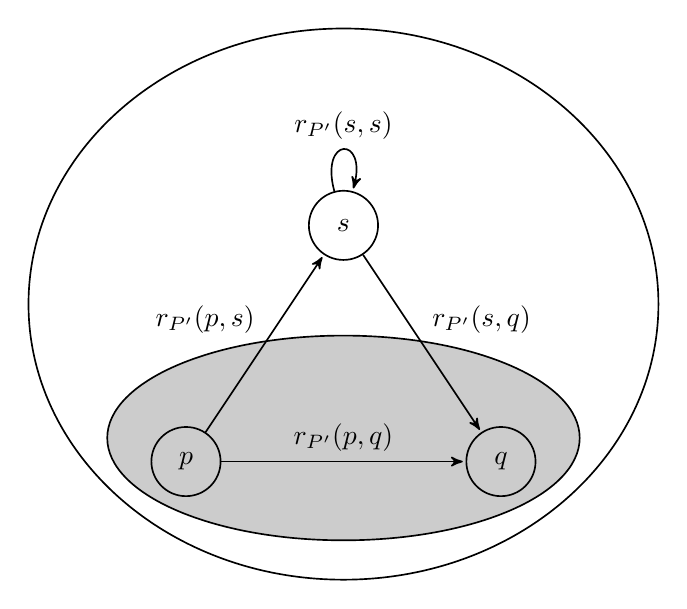
\begin{tikzpicture}[->, >=stealth', shorten >=1pt, auto, semithick]
		\draw[black, fill=black!20] (2, .3) circle[x radius=3, y radius= 1.3];
		\draw[black] (2, 2) circle[x radius=4, y radius=3.5];
		
		\node[state] (p) at (0, 0) {$p$};
		\node[state] (q) at (4, 0) {$q$};
		\node[state] (s) at (2, 3) {$s$};
		
		\path (p) edge node {$r_{P^\prime}(p, q)$} (q)
			(p) edge node {$r_{P^\prime}(p, s)$} (s)
			(s) edge[loop above] node {$r_{P^\prime}(s, s)$} (s) % curly loop
			(s) edge node {$r_{P^\prime}(s, q)$} (q);
	\end{tikzpicture}
	\caption{Rekursionsschritt um einen Zustand rauszuwerfen. Die grau getönte Fläche ist \( P^\prime := P \setminus \{ s \} \). Die größere Fläche ist \( P \). Wichtig: Die Kanten in diesem Graphen sind keine Transitionen, sondern sind mit einem regulären Ausdruck beschriftet, der die Sprache zwischen den Knoten beschreibt mit Zuständen aus dem Index!}
	\label{fig:fwa}
\end{figure}
Falls das Verfahren jemanden bekannt vorkommt, könnte derjenige damit richtig liegen. Es handelt sich bei dem Algorithmus um eine Version des \textit{Floyd-Warshall-Algorithmus}, der in ''Datenstrukturen und Algorithmen`` in der Regel auch vorgestellt wird um günstigste Pfade in gewichteten Graphen zu finden.\par
Die Aufgabe selbst gehe ich jetzt nicht komplett durch, aber ein paar Rekursionsschritte sollten genügen um die idee zu verstehen.
\begin{figure}[h]
	\centering
	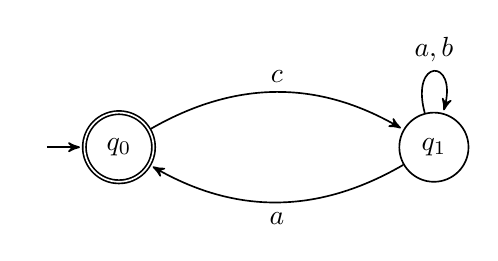
\begin{tikzpicture}[->, >=stealth', shorten >=1pt, auto, semithick]
		\node[state, initial, accepting, initial text=] (q0) at (0, 0) {$q_0$};
		\node[state] (q1) at (4, 0) {$q_1$};
		
		\path (q0) edge[bend left] node {$c$} (q1)
        (q1) edge[loop above] node {$a, b$} (q1)
		(q1) edge[bend left] node {$a$} (q0);   
	\end{tikzpicture}
\end{figure}
Wir suchen also einen regulären Ausdruck, der die Worte beschreibt mit denen man von \( q_0 \) nach \( q_0 \) kommt mit allen Zuständen, also den Ausdruck \( r_Q(q_0, q_0) \). Wir wählen zunächst \( s = q_1 \) (eliminieren \( q_1 \)):
\[
	r_Q(q_0, q_0) = r_{\{ q_0 \}}(q_0, q_0) + r_{\{ q_0 \}}(q_0, q_1) r_{\{ q_0 \}}(q_1, q_1)^\ast r_{\{ q_0 \}}(q_1, q_0)
\]
Noch zu berechnen sind also \( r_{\{ q_0 \}}(q_0, q_0), r_{\{ q_0 \}}(q_0, q_1), r_{\{ q_0 \}}(q_1, q_1), r_{\{ q_0 \}}(q_1, q_0) \). Wir berechnen \( r_{\{ q_0 \}}(q_0, q_0) \) und eliminieren jetzt auch \( q_0 \) und können dann direkt den Basisfall einsetzen:
\begin{align*}
	r_{\{ q_0 \}}(q_0, q_0) &= r_\emptyset(q_0, q_0) + r_\emptyset(q_0, q_0) r_\emptyset(q_0, q_0)^\ast r_\emptyset(q_0, q_0)\\
	&\equiv \varepsilon + \varepsilon \varepsilon^\ast \varepsilon\\
	&\equiv \varepsilon.
\end{align*}
Wir berechnen nun \( r_{\{ q_0 \}}(q_0, q_1) \) und eliminieren wieder \( q_0 \):
\begin{align*}
	r_{\{ q_0 \}}(q_0, q_1) &= r_\emptyset(q_0, q_1) + r_\emptyset(q_0, q_0) r_\emptyset(q_0, q_0)^\ast r_\emptyset(q_0, q_1)\\
	&\equiv c + \varepsilon \varepsilon^\ast c\\
	&\equiv c.
\end{align*}
Die letzten beiden lasse ich mal weg, damit die Aufgabe in späteren Jahrgängen noch verwendet werden kann. Die erhaltenen regulären Ausdrücke lassen sich aber später rekursiv wieder zusammensetzen und man erhält vereinfacht (falls ihr das noch selber machen wollt als Überprüfung):
\[
	r_Q(q_0, q_0) = \varepsilon + c(a+b+ac)^\ast a.
\]


\subsection*{Von regulären Ausdrücken zu Automaten (Thompson-Konstruktion)}
Die andere Richtung, von regulären Ausdrücken zu endlichen Automaten ist deutlich bequemer mit der \textit{Thompson-Konstruktion}. Eine Variante davon wurde in der Vorlesung vorgestellt. Durch die rekursive Definition von regulären Ausdrücken lässt sich aus einem Ausdruck auch rekursiv ein \(\varepsilon\)-NFA aufbauen:\\
Basisfälle:
\begin{figure}[h]
	\begin{minipage}{.3\textwidth}
	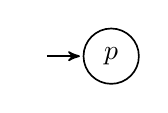
\begin{tikzpicture}[->, >=stealth', shorten >=1pt, auto, semithick, every state/.style={inner sep=0pt, minimum size=20pt}]
		\node[state, initial, initial text=] (0) at (0, 0) {$p$};
	\end{tikzpicture}
	\caption{\( r = \emptyset \)}
	\end{minipage}
	\begin{minipage}{.3\textwidth}
	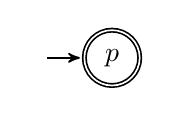
\begin{tikzpicture}[->, >=stealth', shorten >=1pt, auto, semithick, every state/.style={inner sep=0pt, minimum size=20pt}]
		\node[state, initial, initial text=, accepting] (0) at (0, 0) {$p$};
	\end{tikzpicture}
	\caption{\( r = \varepsilon \)}
	\end{minipage}
	\begin{minipage}{.3\textwidth}
	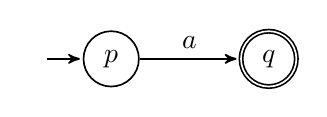
\begin{tikzpicture}[->, >=stealth', shorten >=1pt, auto, semithick, every state/.style={inner sep=0pt, minimum size=20pt}]
		\node[state, initial, initial text=] (0) at (0, 0) {$p$};
		\node[state, accepting] (1) at (2, 0) {$q$};
		
		\path (0) edge node {$a$} (1);
	\end{tikzpicture}
	\caption{\( r = a \)}
	\end{minipage}
\end{figure}\\
Rekursive Fälle: Seien \( \mathcal{A}_e, \mathcal{A}_{e^\prime} \) \( \varepsilon \)-NFAs für die regulären Ausdrücke \( e, e^\prime \) mit Startzuständen \( q_0, q_0^\prime \) und (verinfachte Darstellung mit nur einem Endzustand) akzeptierenden Zuständen \( q_f, q_f^\prime \). In den Abbildungen~\ref{fig:plus},~\ref{fig:dot} und~\ref{fig:star} ist dargestellt wie die Komposition mit \( +, \cdot und ^\ast \) funktioniert.
\begin{figure}[h]
	\begin{minipage}{.5\textwidth}
	\centering
	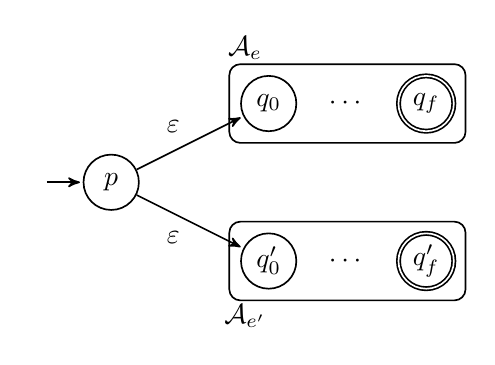
\begin{tikzpicture}[->, >=stealth', shorten >=1pt, auto, semithick, every state/.style={inner sep=0pt, minimum size=20pt}]
		\node[state, initial, initial text=] (0) at (0, 0) {$p$};
		
		\node at (1.7, 1.7) {$\mathcal{A}_e$};
		\draw[black, rounded corners] (1.5, 1.5) rectangle (4.5, .5);
		\node[state] (1) at (2, 1) {$q_0$};
		\node[state, accepting] (2) at (4, 1) {$q_f$};
		\node (d1) at (3, 1) {$\cdots$};
		
		\node at (1.7, -1.7) {$\mathcal{A}_{e^\prime}$};
		\draw[black, rounded corners] (1.5, -1.5) rectangle (4.5, -.5);
		\node[state] (3) at (2, -1) {$q_0^\prime$};
		\node[state, accepting] (4) at (4, -1) {$q_f^\prime$};
		\node (d2) at (3, -1) {$\cdots$};
		
		\path (0) edge node {$\varepsilon$} (1)
			(0) edge node[below left] {$\varepsilon$} (3);	
	\end{tikzpicture}
	\caption{\( r = e + e^\prime \)}
	\label{fig:plus}
	\end{minipage}
	\begin{minipage}{.5\textwidth}
	\centering
	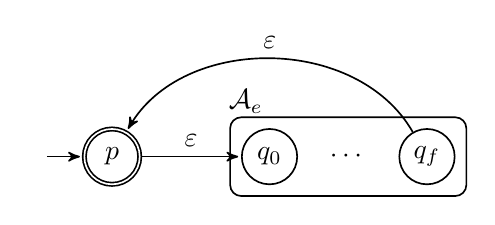
\begin{tikzpicture}[->, >=stealth', shorten >=1pt, auto, semithick, every state/.style={inner sep=0pt, minimum size=20pt}]
		\node[state, initial, initial text=, accepting] (0) at (0, 0) {$p$};
		
		\node at (1.7, .7) {$\mathcal{A}_e$};
		\draw[black, rounded corners] (1.5, .5) rectangle (4.5, -.5);
		\node[state] (1) at (2, 0) {$q_0$};
		\node[state] (2) at (4, 0) {$q_f$};
		\node (d1) at (3, 0) {$\cdots$};
		
		\path (0) edge node {$\varepsilon$} (1)
			(2) edge[bend right=60] node[above] {$\varepsilon$} (0);
		
	\end{tikzpicture}
	\caption{\( r = e^\ast \)}
	\label{fig:star}
	\end{minipage}
\end{figure}
\begin{figure}[h]
	\centering
	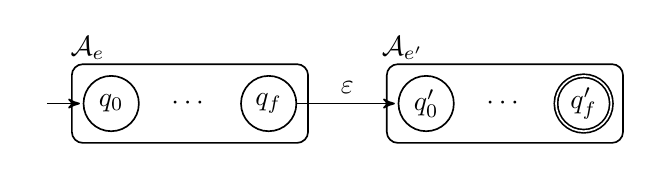
\begin{tikzpicture}[->, >=stealth', shorten >=1pt, auto, semithick, every state/.style={inner sep=0pt, minimum size=20pt}]
		\node at (1.7, .7) {$\mathcal{A}_e$};
		\draw[black, rounded corners] (1.5, .5) rectangle (4.5, -.5);
		\node[initial, initial text=, state] (1) at (2, 0) {$q_0$};
		\node[state] (2) at (4, 0) {$q_f$};
		\node (d1) at (3, 0) {$\cdots$};
		
		\node at (5.7, .7) {$\mathcal{A}_{e^\prime}$};
		\draw[black, rounded corners] (5.5, .5) rectangle (8.5, -.5);
		\node[state] (3) at (6, 0) {$q_0^\prime$};
		\node[state, accepting] (4) at (8, 0) {$q_f^\prime$};
		\node (d2) at (7, 0) {$\cdots$};
		
		\path (2) edge node {$\varepsilon$} (3);
		
	\end{tikzpicture}
	\caption{\( r = e \cdot e^\prime \)}
	\label{fig:dot}
\end{figure}
Es entstehen viele überflüssige \(\varepsilon\)-Transitionen, in der Hausaufgabe sollten diese aber besser nicht weggelassen werden. Die Konstruktion funktioniert immer und ist auch leichter zu implementieren als vielleicht effizientere Ansätze, die in FoSAP nicht behandelt werden.\par
Ein Minimalbeispiel:
\[
	r = (a+b)^\ast c.
\]
Die Automaten für die Teilausdrücke \( a, b, c \) sind klar, wir starten mit \( (a+b) \) in Abbildung~\ref{fig:re1}.
\begin{figure}[h]
	\centering
	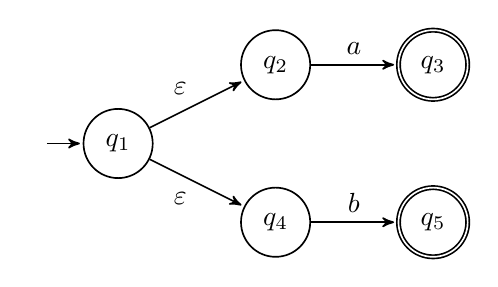
\begin{tikzpicture}[->, >=stealth', shorten >=1pt, auto, semithick]
		\node[state, initial, initial text=] (1) at (0, 0) {$q_1$};
		\node[state] (2) at (2, 1) {$q_2$};
		\node[state, accepting] (3) at (4, 1) {$q_3$};
		\node[state] (4) at (2, -1) {$q_4$};
		\node[state, accepting] (5) at (4, -1) {$q_5$};
		
		\path (1) edge node {$\varepsilon$} (2)
			(1) edge node[below left] {$\varepsilon$} (4)
			(2) edge node {$a$} (3)
			(4) edge node {$b$} (5);
	\end{tikzpicture}
	\caption{NFA für \( (a + b) \)}
	\label{fig:re1}
\end{figure}
Um den Kleene'schen Abschluss zu bilden ergänzen wir einen (eigentlich überflüssigen, aber nach Konstruktion erforderlichen) Zustand \( q_0^\ast \), der neuer Startzustand wird und akzeptierend wird. Die ursprünglichen akzeptierenden Zustände werden nicht-akzeptierend und bekommen Transitionen zum neuen Startzustand.
\begin{figure}[h]
	\centering
	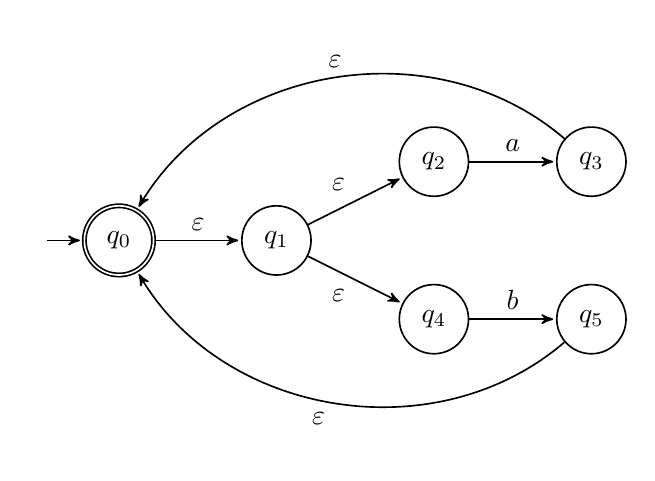
\begin{tikzpicture}[->, >=stealth', shorten >=1pt, auto, semithick]
		\node[state, initial, initial text=, accepting] (0) at (-2, 0) {$q_0$};
		\node[state] (1) at (0, 0) {$q_1$};
		\node[state] (2) at (2, 1) {$q_2$};
		\node[state] (3) at (4, 1) {$q_3$};
		\node[state] (4) at (2, -1) {$q_4$};
		\node[state] (5) at (4, -1) {$q_5$};
		
		\path (0) edge node {$\varepsilon$} (1)
			(1) edge node {$\varepsilon$} (2)
			(1) edge node[below left] {$\varepsilon$} (4)
			(2) edge node {$a$} (3)
			(4) edge node {$b$} (5)
			(3) edge[bend right=50] node[above] {$\varepsilon$} (0)
			(5) edge[bend left=50] node {$\varepsilon$} (0);
	\end{tikzpicture}
	\caption{NFA für \( (a + b)^\ast \)}
	\label{fig:re2}
\end{figure}
Zuletzt die Konkatenation von \( c \): Dazu fügen wir eine \(\varepsilon\)-Transition vom (noch) akzeptierenden Zustand vom Automaten in Abbildung~\ref{fig:re2} zum Startzustand des trivialen Automaten für die Sprache \( \{ c \} \). Der fertige Automat ist in Abbildung~\ref{fig:re3}.
\begin{figure}[h]
	\centering
	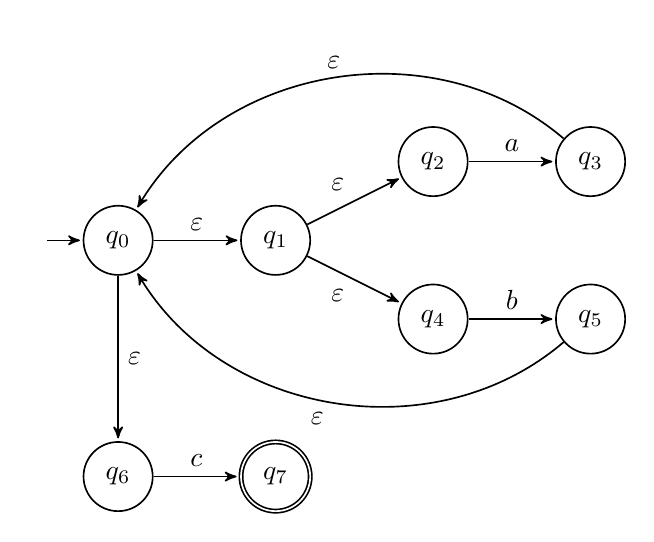
\begin{tikzpicture}[->, >=stealth', shorten >=1pt, auto, semithick]
		\node[state, initial, initial text=] (0) at (-2, 0) {$q_0$};
		\node[state] (1) at (0, 0) {$q_1$};
		\node[state] (2) at (2, 1) {$q_2$};
		\node[state] (3) at (4, 1) {$q_3$};
		\node[state] (4) at (2, -1) {$q_4$};
		\node[state] (5) at (4, -1) {$q_5$};
		\node[state] (6) at (-2, -3) {$q_6$};
		\node[state, accepting] (7) at (0, -3) {$q_7$};
		
		\path (0) edge node {$\varepsilon$} (1)
			(1) edge node {$\varepsilon$} (2)
			(1) edge node[below left] {$\varepsilon$} (4)
			(2) edge node {$a$} (3)
			(4) edge node {$b$} (5)
			(3) edge[bend right=50] node[above] {$\varepsilon$} (0)
			(5) edge[bend left=50] node {$\varepsilon$} (0)
			(0) edge node {$\varepsilon$} (6)
			(6) edge node {$c$} (7);
	\end{tikzpicture}
	\caption{NFA für \( (a + b)^\ast c \)}
	\label{fig:re3}
\end{figure}
In den Hausaufgaben müsst ihr das nicht so ausführlich machen. Es reicht der Automat der Am Ende rauskommt. Ihr sollt aber das Verfahren aus der Vorlesung benutzen. Der Automat in Abbildung~\ref{fig:ref} ist zwar viel kleiner und äquivalent, aber nicht zulässig.
\begin{figure}
	\centering
	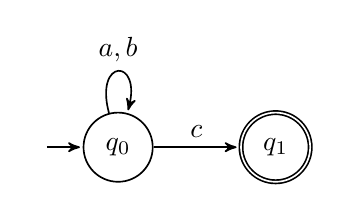
\begin{tikzpicture}[->, >=stealth', shorten >=1pt, auto, semithick]
		\node[state, initial, initial text=] (0) at (0, 0) {$q_0$};
		\node[state, accepting] (1) at (2, 0) {$q_1$};
		
		\path (0) edge[loop above] node {$a, b$} (0)
			(0) edge node {$c$} (1);
	\end{tikzpicture}
	\caption{Ein minimaler NFA für die Sprache \( L((a+b)^\ast c) \).}
	\label{fig:ref}
\end{figure}

\subsection*{Nicht-reguläre Sprachen (Pumping-Argument)}
Dies ist eine Aufgabe mit der Studenten in der Regel Probleme haben, da das Pumping-Lemma etwas sperrig ist und nicht sehr natürlich wirkt. Zur Erinnerung aber trotzdem nochmal:\par
Sei \( L \) eine reguläre Sprache. Dann existiert ein \( n \in \mathbb{N}_+ \), sodass für alle \( w \in L \) mit \( \left| w \right| \geq n \) eine Zerlegung \( w = xyz \) existiert für die gilt:
\begin{enumerate}
	\item \( \left| xy \right| \leq n \),
	\item \( y \neq \varepsilon \),
	\item \( xy^i z \in L \) für alle \( i \in \mathbb{N} \).
\end{enumerate}
Wir betrachten jetzt die Sprache 
\[
	L = \{ uav \,\vert\, u, v \in \{ a, b \}^\ast \text{ mit } \left| u \right| = \left| v \right| \} 
\]
Der herkömmliche Weg, der auch in der Vorlesung vorgestellt wurde ist nun genau dieses Lemma benutzen und die Annahme, dass \( L \) regulär ist zu einem Widerspruch zu führen. Das ist aber genau das womit viele Schwierigkeiten haben, deswegen versuche ich das hier etwas anschaulicher:\par
Angenommen \( L \) ist regulär, dann gibt es einen endlichen Automaten \( \mathcal{A} = (Q, \Sigma, \Delta, q_0, F) \), der \( L \) erkennt. Angenommen \( \mathcal{A} \) habe \( n \) Zustände. Wir betrachten das Wort \( w = b^n a b^n \). Das Wort ist in der Sprache und hat die Länge \( 2n+1 > n \). Nach Lesen des Präfix \( b^n \) muss also spätestens eine Zustandswiederholung im akzeptierenden Lauf von \( \mathcal{A} \) auf \( w \) aufgetreten sein (\textit{pigeonhole principle, Schubfachprinzip}), d.h. vor dem Lesen vom \( a \). Wir nehmen an, der Zustand, der sich wiederholt trat nach Lesen des \(i\)-ten und \(j\)-ten (oBdA \( j > i \)) \( b \) auf (s. Abbildung~\ref{fig:pl}). Wir betrachten also den Lauf
\[
	r = (q_0, b,  q_1, \ldots, b, q_i, b, \ldots, q_j, b, q_{j+1}, \ldots, b, q_n, a, q_{n+1}, b, \ldots, b, q_{2n+1}),
\]
mit \( q_{2n+1} \in F \) wobei \( q_i = q_j \). Sei \( j-i = k > 0 \). Der Lauf 
\[
	r = (q_0, b, \ldots, q_i, b, q_{j+1}, \ldots, b, q_{2n+1})
\]
ist also ebenfalls möglich und auch akzeptierend mit dem Wort \( w^\prime = b^{n-k}ab^n \), aber \( w^\prime \notin L \), also erkennt \( \mathcal{A} \) nicht die Sprache mit \( n \) Zuständen. Da \( n \) beliebig war gibt es also keinen endlichen Automaten, der \( L \) akzeptiert. Somit folgt, dass \( L \) nicht regulär ist.\par
Man sieht vielleicht, dass in dieser Lösung die Wörter und Zahlen aus dem Pumping Lemma wieder auftauchen, was natürlich kein Zufall ist (\( n \), Das Präfix \( b^j \) entspricht \( xy \), das Infix \( b^k \) mit \( k > 0 \) entspricht \( y \) und das Weglassen von \( b^k \) in \( w^\prime \) entspricht der Betrachtung von \( xz \) in \textit{iii)}).\\
Es wird in Zukunft noch weitere Aufgaben dieses Typs geben. Vor der Präsenzübung wird darauf auch im Tutorium nochmal eingegangen.
\begin{figure}
	\centering
	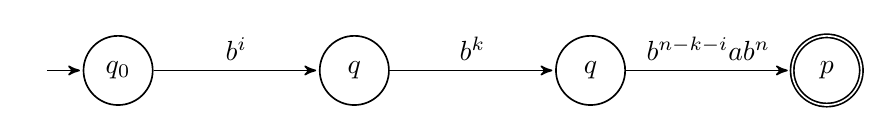
\begin{tikzpicture}[->, >=stealth', shorten >=1pt, auto, semithick]
		\node[state, initial, initial text=] (0) at (0, 0) {$q_0$};
		\node[state] (i) at (3, 0) {$q$};
		\node[state] (j) at (6, 0) {$q$};
		\node[state, accepting] (p) at (9, 0) {$p$};
		
		\path (0) edge node {$b^i$} (i)
			(i) edge node {$b^k$} (j)
			(j) edge node {$b^{n-k-i}ab^n$} (p);
	\end{tikzpicture}
	\caption{Zustandswiederholung in \( q \). Es gibt also einen Lauf von \( q_0 \) nach \( q \) und einen Lauf von \( q \) nach \( p \). Den Zwischenlauf von \( q \) nach \( q \) kann man also weglassen (oder auch beliebig oft wiederholen).}
	\label{fig:pl}
\end{figure}

\end{document}